% =====================================================================
%  Rapport technique — TRS & maintenance predictive
%  Compilation : xelatex rapport.tex (deux passes) ou tectonic rapport.tex
% =====================================================================
\documentclass[11pt,a4paper]{article}

% ---------- Langue et polices ----------
\usepackage{fontspec}
\usepackage{unicode-math}
\setmainfont{texgyrepagella}[Extension=.otf, UprightFont=*-regular, BoldFont=*-bold,
  ItalicFont=*-italic, BoldItalicFont=*-bolditalic]
\setsansfont{texgyreheros}[Extension=.otf, UprightFont=*-regular, BoldFont=*-bold,
  ItalicFont=*-italic, BoldItalicFont=*-bolditalic]
\setmonofont{lmmono10-regular}[Extension=.otf, Scale=0.95]
\setmathfont{texgyrepagella-math.otf}
\usepackage[french]{babel}
\usepackage{microtype}

% ---------- Mise en page ----------
\usepackage[a4paper,top=2.5cm,bottom=2.6cm,left=2.5cm,right=2.5cm,headheight=14pt]{geometry}
\usepackage{xcolor}
\definecolor{navy}{HTML}{1B2A4A}
\definecolor{slate}{HTML}{3D5A80}
\definecolor{accent}{HTML}{E07A5F}
\definecolor{muted}{HTML}{6B7785}
\definecolor{fond}{HTML}{F4F6F9}
\definecolor{vert}{HTML}{2D6A4F}
\definecolor{rouge}{HTML}{C1292E}

\usepackage{graphicx}
\usepackage{booktabs}
\usepackage{tabularx}
\usepackage{array}
\usepackage{multirow}
\usepackage{amsmath}
\usepackage{enumitem}
\setlist{itemsep=2pt,topsep=4pt}
\usepackage[font=small,labelfont={bf,color=navy},labelsep=period]{caption}
\usepackage{tikz}
\usetikzlibrary{positioning,arrows.meta,shapes.misc}
\usepackage[most]{tcolorbox}

\usepackage{titlesec}
\titleformat{\section}{\sffamily\Large\bfseries\color{navy}}{\thesection}{0.8em}{}
\titleformat{\subsection}{\sffamily\large\bfseries\color{navy}}{\thesubsection}{0.7em}{}
\titleformat{\subsubsection}{\sffamily\normalsize\bfseries\color{slate}}{\thesubsubsection}{0.6em}{}
\titlespacing*{\section}{0pt}{18pt}{8pt}
\titlespacing*{\subsection}{0pt}{12pt}{5pt}

\usepackage{fancyhdr}
\pagestyle{fancy}
\fancyhf{}
\fancyhead[L]{\sffamily\footnotesize\color{muted}TRS \& maintenance prédictive}
\fancyhead[R]{\sffamily\footnotesize\color{muted}\leftmark}
\fancyfoot[C]{\sffamily\footnotesize\color{muted}\thepage}
\renewcommand{\headrulewidth}{0.4pt}
\renewcommand{\headrule}{\hbox to\headwidth{\color{fond!60!muted}\leaders\hrule height \headrulewidth\hfill}}
\renewcommand{\sectionmark}[1]{\markboth{#1}{}}

\usepackage[hidelinks]{hyperref}
\hypersetup{pdftitle={TRS et maintenance prédictive — Rapport technique},
            pdfauthor={KOUTSAVA Kossi Epiphane}}

% ---------- Encadres ----------
\newtcolorbox{encadre}[1][]{enhanced,breakable,colback=fond,colframe=fond,
  borderline west={3pt}{0pt}{accent},arc=2pt,left=10pt,right=10pt,top=6pt,bottom=6pt,
  fonttitle=\sffamily\bfseries\small,coltitle=accent,
  title={#1},attach title to upper={\par\smallskip}}
\newtcolorbox{retenir}{enhanced,colback=navy!4,colframe=navy!4,
  borderline west={3pt}{0pt}{navy},arc=2pt,left=10pt,right=10pt,top=6pt,bottom=6pt}

\newcommand{\code}[1]{\texttt{#1}}
\newcommand{\pct}[1]{#1~\%}

% =====================================================================
\begin{document}

% ---------- Page de garde ----------
\begin{titlepage}
\setlength{\parindent}{0pt}
\newcommand{\infogarde}[2]{\makebox[4.6cm][l]{\sffamily\color{muted}#1}#2\par\vspace{5pt}}
\begin{tikzpicture}[remember picture,overlay]
  \fill[navy] (current page.north west) rectangle ([yshift=-11.5cm]current page.north east);
  \fill[accent] ([yshift=-11.5cm]current page.north west) rectangle ([yshift=-11.75cm]current page.north east);
\end{tikzpicture}
\vspace*{0.4cm}
{\sffamily\color{accent!60!white}\small\bfseries MASTER 1 BIG DATA \textperiodcentered{} UCAO-UUT\par}
\vspace{1.4cm}
{\sffamily\color{white}\fontsize{28}{34}\selectfont\bfseries
Taux de Rendement Synthétique\\[2pt] et maintenance prédictive\par}
\vspace{0.6cm}
{\sffamily\color{white!80!navy}\Large Atelier de production — Zone Franche du Togo\par}
\vspace{0.35cm}
{\sffamily\color{white!65!navy}\large Rapport technique : données, modèles, entraînement et évaluation\par}

\vspace{3.6cm}
\infogarde{Auteur}{KOUTSAVA Kossi Epiphane}
\infogarde{Formation}{Master 1 Big Data — UCAO-UUT}
\infogarde{Unité d'enseignement}{INF2224 — Extraction d'Information}
\infogarde{Code source}{\href{https://github.com/kkepiphane/trs-zone-franche-tg}{\small\code{github.com/kkepiphane/trs-zone-franche-tg}}}
\infogarde{Date}{Octobre 2026}

\vfill
\begin{encadre}[À propos des données]
Les données de production industrielles étant confidentielles, ce travail s'appuie sur un
\textbf{jeu de données simulé de façon réaliste}, avec un scénario de dégradation contrôlé.
Les résultats chiffrés illustrent et valident la démarche ; ils ne constituent pas une mesure
de performance sur un atelier réel.
\end{encadre}
\end{titlepage}

% ---------- Resume ----------
\section*{Résumé}
\addcontentsline{toc}{section}{Résumé}
Ce rapport décrit une chaîne de traitement de données complète, de la donnée brute de production
jusqu'à la prédiction, appliquée au suivi d'un atelier de cinq machines. La performance est mesurée
par le \textbf{Taux de Rendement Synthétique} (TRS), produit de la disponibilité, de la performance
et de la qualité. Deux modèles d'apprentissage sont construits : une \textbf{régression linéaire}
qui projette la tendance du TRS de chaque machine, et une \textbf{forêt aléatoire} (Random Forest)
qui estime la probabilité qu'une défaillance survienne dans les cinq jours ouvrés suivants, à partir
d'indicateurs calculés sur une fenêtre glissante.

Sur le jeu simulé (450 relevés journaliers, TRS global de \pct{79,3}), la machine M-03 est
identifiée comme critique : tendance de $-0{,}31$ point de TRS par jour ($R^2 = 0{,}79$) et
probabilité de panne estimée à \pct{90}. Sur le jeu de test, le classifieur obtient une exactitude
de \pct{98,3} mais un rappel de \pct{33} au seuil de décision par défaut. L'analyse montre que
l'exactitude est trompeuse sur des classes aussi déséquilibrées (\pct{2,25} de cas positifs), que
le classement des risques est en réalité parfait (AUC~$=1$) et qu'un seuil de $0{,}2$ permet de
détecter toutes les pannes du test au prix d'une fausse alerte. Les limites liées à la taille de
l'échantillon et au découpage des données sont discutées. L'ensemble est livré dans un tableau de
bord interactif (Plotly Dash).

\vspace{0.4cm}
\noindent{\sffamily\small\color{muted}\textbf{Mots-clés :} TRS, OEE, maintenance prédictive,
Random Forest, classes déséquilibrées, régression linéaire, tableau de bord.}

\newpage
\tableofcontents
\newpage

% =====================================================================
\section{Introduction}

\subsection{Contexte}
Dans les entreprises industrielles de la Zone Franche du Togo, comme dans toute industrie
manufacturière, un arrêt machine non planifié se traduit par de la production perdue, des
retards de livraison et des coûts d'intervention en urgence. Trois stratégies de maintenance
coexistent :
\begin{itemize}
  \item la maintenance \textbf{corrective}, qui intervient après la panne ;
  \item la maintenance \textbf{préventive}, qui intervient à intervalles fixes, que la machine
        en ait besoin ou non ;
  \item la maintenance \textbf{prédictive}, qui intervient lorsque les données indiquent
        qu'une défaillance devient probable.
\end{itemize}
La maintenance prédictive suppose de disposer de données de production, d'un indicateur de
performance fiable et de modèles capables d'anticiper une dégradation. C'est l'objet de ce projet.

\subsection{Objectifs}
\begin{enumerate}
  \item \textbf{Mesurer} la performance de chaque machine par le TRS et ses trois composantes.
  \item \textbf{Diagnostiquer} la composante qui pénalise le plus chaque machine.
  \item \textbf{Prévoir} l'évolution du TRS à court terme.
  \item \textbf{Prédire} le risque de défaillance de chaque machine dans les jours qui suivent.
  \item \textbf{Restituer} ces résultats dans un outil d'aide à la décision utilisable par un
        responsable de production.
\end{enumerate}

\subsection{Démarche}
La figure~\ref{fig:pipeline} résume la chaîne de traitement. L'exploration et l'entraînement
sont réalisés dans un notebook Jupyter ; le modèle obtenu est exporté puis chargé par le tableau
de bord, selon la séparation usuelle entre expérimentation et mise en production.

\begin{figure}[ht]
\centering
\begin{tikzpicture}[
  node distance=0.45cm,
  etape/.style={rounded rectangle, draw=navy, line width=0.8pt, fill=white,
                minimum height=1.05cm, minimum width=2.45cm, align=center,
                font=\sffamily\small},
  num/.style={circle, fill=navy, text=white, font=\sffamily\scriptsize\bfseries,
              inner sep=1.5pt, minimum size=0.42cm},
  fl/.style={-{Stealth[length=2.4mm]}, line width=0.8pt, color=slate}]
  \node[etape] (a) {\textbf{Ingestion}\\[-1pt]{\scriptsize\color{muted}CSV, schéma}};
  \node[etape, right=of a] (b) {\textbf{Préparation}\\[-1pt]{\scriptsize\color{muted}nettoyage}};
  \node[etape, right=of b] (c) {\textbf{Analyse TRS}\\[-1pt]{\scriptsize\color{muted}KPI, diagnostic}};
  \node[etape, right=of c, draw=accent] (d) {\textbf{Prédiction}\\[-1pt]{\scriptsize\color{muted}régression, RF}};
  \draw[fl] (a) -- (b); \draw[fl] (b) -- (c); \draw[fl] (c) -- (d);
  \foreach \n/\k in {a/1,b/2,c/3,d/4} \node[num] at (\n.north west) {\k};
  \node[below=0.55cm of b.south east, font=\sffamily\scriptsize, color=muted, align=center]
    (t) {\code{calcul\_trs.py} \quad·\quad \code{prediction.py} \quad·\quad
         notebook Jupyter \quad·\quad tableau de bord Dash (\code{app.py})};
\end{tikzpicture}
\caption{Chaîne de traitement, de la donnée brute à la prédiction.}
\label{fig:pipeline}
\end{figure}

% =====================================================================
\section{Données}

\subsection{Origine : un jeu simulé au scénario contrôlé}
Les données sont produites par le script \code{generer\_donnees.py} (graine aléatoire fixée à
42, donc reproductibles). Elles décrivent un atelier de \textbf{5 machines} (M-01 à M-05) suivies
pendant \textbf{90 jours ouvrés}, du 02/02/2026 au 05/06/2026, soit \textbf{450 relevés journaliers}.

Chaque machine possède un profil de base (disponibilité, performance, qualité) autour duquel les
valeurs journalières varient selon une loi normale. Une \textbf{dérive} de la disponibilité est
ajoutée : nulle pour M-01, M-02 et M-05, modérée pour M-04 ($-0{,}0015$ par jour) et forte pour
\textbf{M-03} ($-0{,}0032$ par jour). Les signaux d'usure (arrêts, micro-arrêts, température
moteur) sont tirés à partir de la perte de disponibilité, ce qui reproduit le comportement
attendu d'une machine qui se dégrade.

\begin{encadre}[Pourquoi un scénario contrôlé ?]
Connaître à l'avance la machine qui se dégrade permet de \textbf{vérifier} que la chaîne détecte
bien une anomalie connue, avant de l'appliquer à des données réelles. En contrepartie, la relation
entre signaux d'usure et disponibilité est construite par le générateur : le modèle la retrouve
plus facilement qu'il ne le ferait sur des données d'usine (voir section~\ref{sec:limites}).
\end{encadre}

\subsection{Schéma des données}
Le tableau~\ref{tab:schema} décrit les colonnes. Les sept premières sont obligatoires pour calculer
le TRS ; les trois dernières alimentent le modèle de risque de panne.

\begin{table}[ht]
\centering\small
\caption{Schéma du fichier de production (un relevé par machine et par jour).}
\label{tab:schema}
\begin{tabularx}{\textwidth}{@{}l l X@{}}
\toprule
\textbf{Colonne} & \textbf{Unité} & \textbf{Description} \\
\midrule
\code{machine}        & —        & identifiant de la machine \\
\code{date}           & —        & jour de production \\
\code{temps\_prevu}   & min      & temps de production planifié ($T_p$, 450 min par jour) \\
\code{temps\_marche}  & min      & temps de fonctionnement effectif ($T_m$) \\
\code{prod\_theorique}& pièces   & production atteignable à la cadence nominale pendant $T_m$ ($N_{th}$) \\
\code{prod\_reelle}   & pièces   & pièces effectivement produites ($N_r$) \\
\code{pieces\_bonnes} & pièces   & pièces conformes ($N_b$) \\
\midrule
\code{nb\_arrets}     & nombre   & arrêts de la journée \\
\code{micro\_arrets}  & nombre   & arrêts de courte durée \\
\code{temp\_moteur}   & °C       & température moyenne du moteur \\
\bottomrule
\end{tabularx}
\end{table}

\subsection{Préparation et contrôle qualité}
Avant tout calcul, la fonction \code{nettoyer()} applique les règles suivantes :
\begin{enumerate}
  \item suppression des doublons exacts ;
  \item suppression des lignes dont une valeur obligatoire est manquante ;
  \item cohérence physique : $T_m \le T_p$ et $N_b \le N_r$ ;
  \item dénominateurs strictement positifs : $T_p > 0$, $N_{th} > 0$, $N_r > 0$.
\end{enumerate}
Sur le jeu simulé, aucune ligne n'est rejetée (450 sur 450). Ces règles sont néanmoins
indispensables sur des données réelles, saisies manuellement ou issues de capteurs. Le tableau de
bord affiche le nombre de lignes rejetées et les valeurs manquantes à chaque import.

% =====================================================================
\section{Le Taux de Rendement Synthétique}

\subsection{Définition}
Pour une machine et une journée donnée, les trois composantes et le TRS sont définis par :
\begin{equation}
D = \frac{T_m}{T_p}, \qquad
P = \frac{N_r}{N_{th}}, \qquad
Q = \frac{N_b}{N_r}, \qquad
\mathrm{TRS} = D \times P \times Q .
\label{eq:trs}
\end{equation}
La \textbf{disponibilité} $D$ mesure les pertes dues aux arrêts, la \textbf{performance} $P$ les
pertes de cadence (micro-arrêts, ralentissements) et la \textbf{qualité} $Q$ les pertes dues aux
rebuts. Un TRS de \pct{85} est communément retenu comme référence de « classe mondiale » ; c'est
l'objectif fixé dans ce projet.

Le TRS d'une machine sur une période est la moyenne de ses TRS journaliers ; le TRS de l'atelier
est la moyenne sur l'ensemble des relevés. Comme la moyenne d'un produit n'est pas le produit des
moyennes, ce TRS global diffère légèrement du produit des trois composantes moyennes (moins de
0,1~point ici).

\subsection{Résultats}
Le TRS de l'atelier s'établit à \textbf{\pct{79,3}}, soit 5,7~points sous l'objectif.
Trois machines sur cinq sont sous l'objectif (tableau~\ref{tab:trs}, figure~\ref{fig:trs}).

\begin{table}[ht]
\centering\small
\caption{Composantes moyennes et TRS par machine, du plus faible au plus élevé.}
\label{tab:trs}
\begin{tabular}{@{}lcccc@{}}
\toprule
\textbf{Machine} & \textbf{Disponibilité} & \textbf{Performance} & \textbf{Qualité} & \textbf{TRS} \\
\midrule
M-03 & \textcolor{rouge}{\textbf{71,4 \%}} & 94,9 \% & 98,1 \% & \textcolor{rouge}{\textbf{66,5 \%}} \\
M-04 & 83,7 \% & 91,7 \% & 95,8 \% & 73,5 \% \\
M-02 & 89,4 \% & 93,0 \% & 97,2 \% & 80,8 \% \\
M-01 & 93,2 \% & 94,3 \% & 99,0 \% & 86,9 \% \\
M-05 & 93,8 \% & 95,7 \% & 98,8 \% & 88,7 \% \\
\midrule
\textbf{Atelier} & 86,3 \% & 93,9 \% & 97,8 \% & \textbf{79,3 \%} \\
\bottomrule
\end{tabular}
\end{table}

\begin{figure}[ht]
\centering
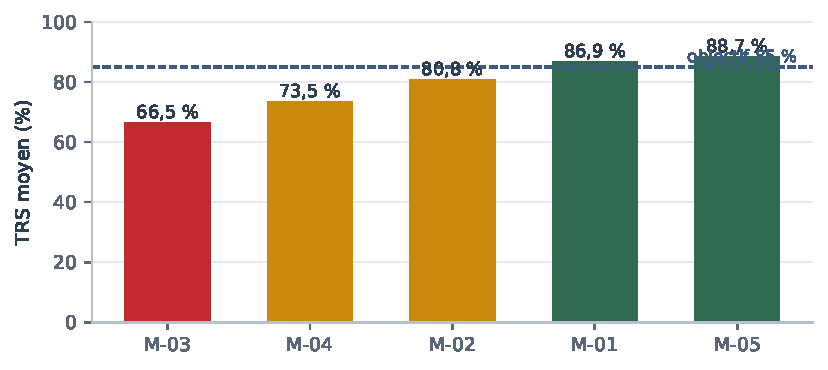
\includegraphics[width=0.86\textwidth]{figures/trs_machines.pdf}
\caption{TRS moyen par machine (vert : objectif atteint ; ocre : entre 70 et \pct{85} ; rouge : sous \pct{70}).}
\label{fig:trs}
\end{figure}

\subsection{Diagnostic}
Pour chaque machine, la composante la plus faible indique où agir en priorité. Pour M-03, c'est
nettement la \textbf{disponibilité} (\pct{71,4}), alors que sa performance et sa qualité sont
comparables à celles des autres machines : la machine \emph{s'arrête} de plus en plus. L'évolution
hebdomadaire (figure~\ref{fig:evol}) confirme une baisse continue, d'environ \pct{80} en février à
environ \pct{53} début juin. M-04 suit la même tendance, de façon plus modérée.

\begin{figure}[ht]
\centering
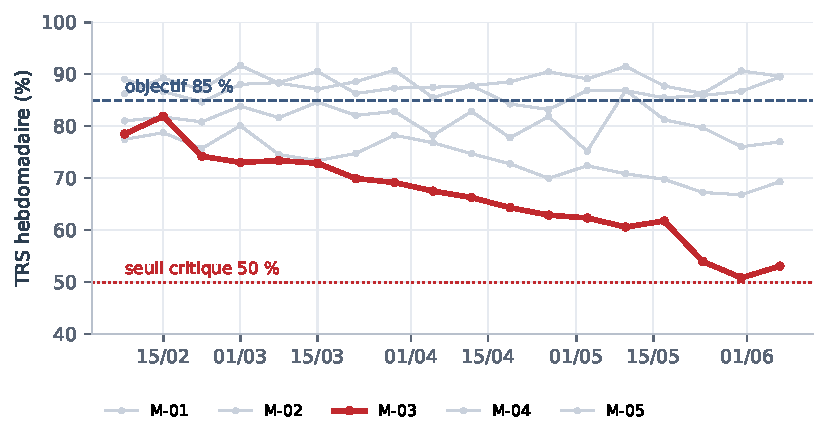
\includegraphics[width=0.86\textwidth]{figures/evolution.pdf}
\caption{Évolution hebdomadaire du TRS. M-03 (en rouge) se rapproche du seuil critique de \pct{50}.}
\label{fig:evol}
\end{figure}

% =====================================================================
\section{Analyse exploratoire}
La matrice de corrélation de Pearson (figure~\ref{fig:corr}) entre les relevés journaliers fait
apparaître deux constats :
\begin{itemize}
  \item le TRS est porté essentiellement par la \textbf{disponibilité} ($r = 0{,}94$), bien plus que
        par la performance ($r = 0{,}38$) ou la qualité ($r = 0{,}33$) ;
  \item les \textbf{arrêts} ($r = -0{,}69$), \textbf{micro-arrêts} ($r = -0{,}71$) et la
        \textbf{température moteur} ($r = -0{,}73$) sont fortement et négativement corrélés au TRS :
        ce sont des \emph{signaux précurseurs} candidats pour la prédiction de panne.
\end{itemize}

\begin{figure}[ht]
\centering
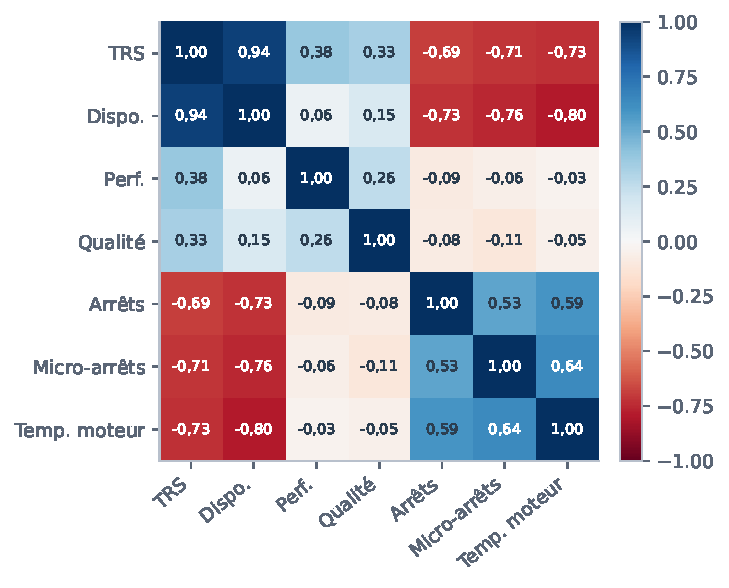
\includegraphics[width=0.56\textwidth]{figures/correlations.pdf}
\caption{Corrélations entre composantes du TRS et signaux d'usure (relevés journaliers).}
\label{fig:corr}
\end{figure}

% =====================================================================
\section{Modèle 1 : prévision de la tendance du TRS}

\subsection{Formulation}
Pour chaque machine, le TRS journalier $y_t$ est modélisé comme une fonction affine du rang $t$ du
jour ouvré ($t = 0, \dots, n-1$) :
\begin{equation}
y_t = \beta_0 + \beta_1\, t + \varepsilon_t .
\end{equation}
Les coefficients sont estimés par moindres carrés ordinaires (\code{LinearRegression} de
scikit-learn), c'est-à-dire en minimisant $\sum_t (y_t - \beta_0 - \beta_1 t)^2$, ce qui donne :
\begin{equation}
\hat\beta_1 = \frac{\sum_t (t-\bar t)(y_t-\bar y)}{\sum_t (t-\bar t)^2}, \qquad
\hat\beta_0 = \bar y - \hat\beta_1 \bar t .
\end{equation}
La pente $\hat\beta_1$ s'interprète directement comme la \textbf{variation du TRS par jour ouvré}.
La projection à l'horizon $h$ est $\hat y_{n-1+h} = \hat\beta_0 + \hat\beta_1 (n-1+h)$, bornée à
$[0, 1]$, et datée sur les jours ouvrés suivants. La qualité de l'ajustement est mesurée par le
coefficient de détermination $R^2 = 1 - \sum_t (y_t-\hat y_t)^2 / \sum_t (y_t-\bar y)^2$.

\subsection{Résultats}
\begin{table}[ht]
\centering\small
\caption{Tendance du TRS par machine (90 jours ouvrés).}
\label{tab:tendance}
\begin{tabular}{@{}lrc l@{}}
\toprule
\textbf{Machine} & \textbf{Pente (pt / jour)} & $\boldsymbol{R^2}$ & \textbf{Lecture} \\
\midrule
M-03 & \textcolor{rouge}{$\mathbf{-0{,}314}$} & \textbf{0,791} & dégradation nette et régulière \\
M-04 & $-0{,}129$ & 0,324 & dégradation modérée \\
M-02 & $-0{,}046$ & 0,058 & stable (pas de tendance significative) \\
M-01 & $-0{,}016$ & 0,007 & stable \\
M-05 & $+0{,}014$ & 0,006 & stable \\
\bottomrule
\end{tabular}
\end{table}

Pour M-03, la droite explique \pct{79} de la variance du TRS : la tendance est à la fois forte et
régulière. Projetée sur 15 jours ouvrés, elle conduit à un TRS de \textbf{\pct{47,8}} et franchit
le seuil critique de \pct{50} au \textbf{9\textsuperscript{e} jour ouvré} (figure~\ref{fig:prev}).
Pour les autres machines, le $R^2$ faible indique que les variations sont dominées par le bruit
journalier : aucune dérive n'est à signaler.

\begin{figure}[ht]
\centering
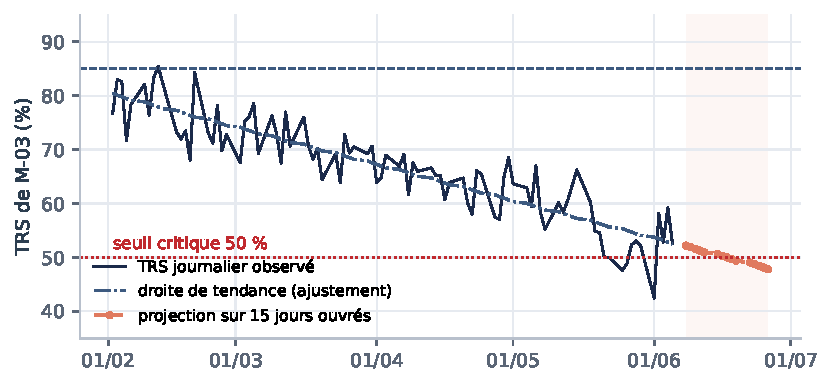
\includegraphics[width=0.88\textwidth]{figures/prevision_m03.pdf}
\caption{TRS journalier de M-03, droite de tendance ajustée et projection sur 15 jours ouvrés.}
\label{fig:prev}
\end{figure}

\begin{retenir}
\textbf{Intérêt opérationnel.} La pente et la date de franchissement du seuil donnent au responsable
de maintenance un \emph{délai d'action} : ici, environ deux semaines pour planifier une intervention
sur M-03 avant que son TRS ne devienne critique.
\end{retenir}

% =====================================================================
\section{Modèle 2 : prédiction du risque de panne}

\subsection{Formulation du problème}
On définit une \textbf{défaillance} comme une journée où le TRS d'une machine passe sous le seuil
critique $s = 0{,}50$. Le problème est posé comme une \textbf{classification binaire supervisée} :
à la date $t$, pour la machine $m$, on cherche à prédire si une défaillance surviendra dans les
$H = 5$ jours ouvrés suivants :
\begin{equation}
y_{m,t} = \begin{cases}
1 & \text{s'il existe } j \in \{t, \dots, t+H-1\} \text{ tel que } \mathrm{TRS}_{m,j} < s,\\
0 & \text{sinon.}
\end{cases}
\end{equation}

\subsection{Construction des variables explicatives}
L'état récent de la machine est résumé sur une \textbf{fenêtre glissante} des $W = 5$ jours
ouvrés \emph{précédant} $t$, notée $\mathcal{F}_t = \{t-W, \dots, t-1\}$. Six variables sont
calculées (tableau~\ref{tab:features}).

\begin{table}[ht]
\centering\small
\caption{Variables explicatives, calculées sur la fenêtre $\mathcal{F}_t$ des 5 jours précédents.}
\label{tab:features}
\begin{tabularx}{\textwidth}{@{}l l X@{}}
\toprule
\textbf{Variable} & \textbf{Calcul} & \textbf{Ce qu'elle capte} \\
\midrule
\code{trs\_moyen}     & moyenne du TRS sur $\mathcal{F}_t$ & niveau de performance récent \\
\code{trs\_pente}     & pente de la droite ajustée au TRS sur $\mathcal{F}_t$ & dégradation en cours \\
\code{dispo\_moyenne} & moyenne de $D$ sur $\mathcal{F}_t$ & pertes par arrêts \\
\code{arrets\_moyens} & moyenne de \code{nb\_arrets} & fréquence des arrêts \\
\code{micro\_moyens}  & moyenne de \code{micro\_arrets} & instabilité de fonctionnement \\
\code{temp\_moyenne}  & moyenne de \code{temp\_moteur} & échauffement, usure mécanique \\
\bottomrule
\end{tabularx}
\end{table}

Les variables n'utilisent que des jours \emph{strictement antérieurs} à $t$, alors que la cible
porte sur les jours $t$ et suivants : aucune information future n'entre dans les variables.

\subsection{Jeu d'apprentissage}
Chaque machine fournit $90 - W - H = 80$ échantillons, soit \textbf{400 échantillons} au total.
Seuls \textbf{9 sont positifs} (\pct{2,25}), tous issus de M-03 : ils correspondent aux fenêtres
qui précèdent les 3 journées où son TRS est passé sous \pct{50}. Les classes sont donc
\textbf{fortement déséquilibrées}, ce qui conditionne tout le reste de la démarche.

\subsection{Séparation apprentissage / test}
Les échantillons sont répartis aléatoirement en \pct{70} pour l'apprentissage et \pct{30} pour
le test (\code{train\_test\_split}, \code{random\_state=42}). La séparation est
\textbf{stratifiée} sur la cible, afin que la proportion de pannes soit la même dans les deux
ensembles ; sans stratification, le jeu de test pourrait ne contenir aucune panne.

\begin{table}[ht]
\centering\small
\caption{Répartition des échantillons.}
\begin{tabular}{@{}lccc@{}}
\toprule
 & \textbf{Échantillons} & \textbf{Pannes} & \textbf{Taux de pannes} \\
\midrule
Apprentissage & 280 & 6 & 2,1 \% \\
Test          & 120 & 3 & 2,5 \% \\
\bottomrule
\end{tabular}
\end{table}

\subsection{Modèle : forêt aléatoire}
\paragraph{Principe.} Une forêt aléatoire combine $B$ arbres de décision. Chaque arbre est appris
sur un échantillon \emph{bootstrap} (tirage avec remise) du jeu d'apprentissage et, à chaque
nœud, ne considère qu'un sous-ensemble aléatoire de variables ($\sqrt{6} \approx 2$ ici). Un nœud
est découpé de façon à réduire au maximum l'\textbf{impureté de Gini} :
\begin{equation}
G = 1 - \sum_{c \in \{0,1\}} p_c^2 ,
\end{equation}
où $p_c$ est la proportion (pondérée) de la classe $c$ dans le nœud. La probabilité de panne
prédite est la moyenne des probabilités données par les $B$ arbres :
$\hat p(x) = \frac{1}{B}\sum_{b=1}^{B} \hat p_b(x)$. La décision est $\hat y = 1$ si
$\hat p(x) \ge \tau$, avec un seuil $\tau = 0{,}5$ par défaut.

Ce modèle a été retenu pour sa robustesse sur de petits jeux de données tabulaires, l'absence
de mise à l'échelle nécessaire, sa capacité à capter des interactions non linéaires et la mesure
d'importance des variables qu'il fournit.

\paragraph{Pondération des classes.} Avec \code{class\_weight="balanced"}, chaque classe reçoit
un poids inversement proportionnel à sa fréquence dans le jeu d'apprentissage :
\begin{equation}
w_c = \frac{n}{K \, n_c}
\quad\Rightarrow\quad
w_0 = \frac{280}{2 \times 274} \approx 0{,}51, \qquad
w_1 = \frac{280}{2 \times 6} \approx 23{,}3 .
\end{equation}
Une erreur sur une panne coûte ainsi environ 46 fois plus qu'une erreur sur un cas sain lors de
la construction des arbres, ce qui compense en partie le déséquilibre.

\begin{table}[ht]
\centering\small
\caption{Hyperparamètres du modèle (\code{RandomForestClassifier}, scikit-learn).}
\label{tab:hyper}
\begin{tabularx}{\textwidth}{@{}l l X@{}}
\toprule
\textbf{Paramètre} & \textbf{Valeur} & \textbf{Justification} \\
\midrule
\code{n\_estimators} & 200 & assez d'arbres pour stabiliser la moyenne des votes \\
\code{max\_depth} & 6 & limite la profondeur pour réduire le surapprentissage sur 280 échantillons \\
\code{class\_weight} & \code{"balanced"} & compense le déséquilibre des classes \\
\code{max\_features} & \code{"sqrt"} (défaut) & décorrèle les arbres \\
\code{criterion} & \code{"gini"} (défaut) & critère de découpage \\
\code{random\_state} & 42 & reproductibilité \\
\bottomrule
\end{tabularx}
\end{table}

\subsection{Évaluation}

\subsubsection{Métriques}
Sur le jeu de test, on compte les vrais positifs ($VP$, pannes détectées), faux positifs ($FP$,
fausses alertes), faux négatifs ($FN$, pannes manquées) et vrais négatifs ($VN$). On en déduit :
\begin{align}
\text{Exactitude} &= \frac{VP + VN}{VP + VN + FP + FN}, &
\text{Précision} &= \frac{VP}{VP + FP}, \\[4pt]
\text{Rappel} &= \frac{VP}{VP + FN}, &
F_1 &= 2\,\frac{\text{Précision} \times \text{Rappel}}{\text{Précision} + \text{Rappel}} .
\end{align}
En maintenance, une panne manquée (arrêt de production) coûte en général bien plus qu'une fausse
alerte (une inspection inutile). Le \textbf{rappel} est donc la métrique prioritaire, la précision
servant à vérifier que les alertes restent crédibles.

\subsubsection{Résultats au seuil par défaut}
\begin{table}[ht]
\centering\small
\caption{Performance sur le jeu de test (120 échantillons, dont 3 pannes), seuil $\tau = 0{,}5$.}
\label{tab:metriques}
\begin{tabular}{@{}lcccc@{}}
\toprule
\textbf{Modèle} & \textbf{Exactitude} & \textbf{Précision} & \textbf{Rappel} & $\boldsymbol{F_1}$ \\
\midrule
Référence naïve : « toujours sain » & 97,5 \% & — & 0 \% & 0 \\
Forêt aléatoire, $\tau = 0{,}5$ & 98,3 \% & 100 \% & \textcolor{rouge}{\textbf{33,3 \%}} & 0,50 \\
\bottomrule
\end{tabular}
\end{table}

Le modèle ne produit aucune fausse alerte, mais il ne détecte qu'\textbf{une panne sur trois}
($VP=1$, $FN=2$, $FP=0$, $VN=117$). L'exactitude de \pct{98,3} est trompeuse : un modèle qui
répondrait toujours « sain » atteindrait déjà \pct{97,5} sans jamais détecter de panne. Sur des
classes aussi déséquilibrées, l'exactitude n'est pas un critère pertinent.

On note aussi un surapprentissage : le modèle classe parfaitement le jeu d'apprentissage
(exactitude et rappel de \pct{100}), ce qui est attendu avec si peu de cas positifs.

\subsubsection{Le seuil de décision, pas le classement}
Les probabilités prédites pour les trois pannes du test sont $0{,}93$, $0{,}39$ et $0{,}23$. Deux
d'entre elles sont sous le seuil de $0{,}5$, mais toutes restent supérieures à celles de l'ensemble
des cas sains : l'aire sous la courbe ROC vaut \textbf{AUC~$=1{,}00$}, de même que la précision
moyenne (AP). Autrement dit, le modèle \emph{classe} parfaitement les situations par niveau de
risque ; c'est le \emph{seuil} de $0{,}5$ qui est inadapté à des probabilités tirées vers le bas
par la rareté des pannes.

\begin{table}[ht]
\centering\small
\caption{Effet du seuil de décision $\tau$ sur le jeu de test.}
\label{tab:seuil}
\begin{tabular}{@{}ccccccc@{}}
\toprule
$\boldsymbol\tau$ & $VP$ & $FN$ & $FP$ & \textbf{Précision} & \textbf{Rappel} & $\boldsymbol{F_1}$ \\
\midrule
0,5 & 1 & 2 & 0 & 100 \% & 33 \% & 0,50 \\
0,3 & 2 & 1 & 0 & 100 \% & 67 \% & 0,80 \\
\textbf{0,2} & \textbf{3} & \textbf{0} & \textbf{1} & \textbf{75 \%} & \textbf{100 \%} & \textbf{0,86} \\
\bottomrule
\end{tabular}
\end{table}

\begin{figure}[ht]
\centering
\begin{minipage}{0.47\textwidth}\centering
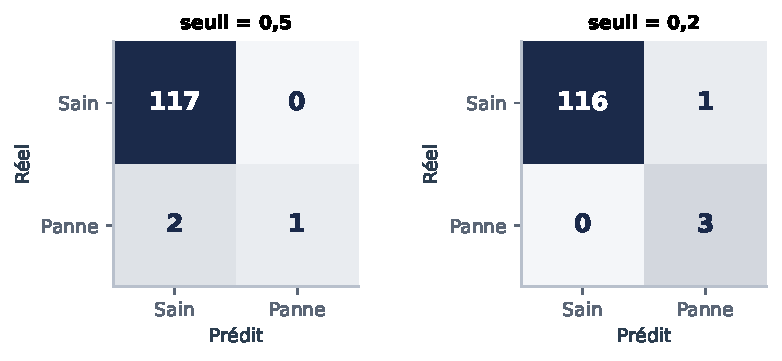
\includegraphics[width=\textwidth]{figures/confusion.pdf}
\end{minipage}\hfill
\begin{minipage}{0.5\textwidth}\centering
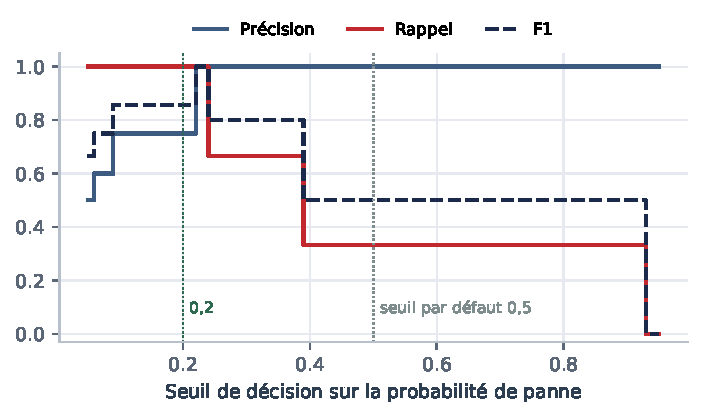
\includegraphics[width=\textwidth]{figures/seuil.pdf}
\end{minipage}
\caption{À gauche : matrices de confusion du jeu de test pour $\tau = 0{,}5$ et $\tau = 0{,}2$.
À droite : précision, rappel et $F_1$ en fonction du seuil.}
\label{fig:seuil}
\end{figure}

Avec $\tau = 0{,}2$, \textbf{les trois pannes sont détectées} au prix d'une seule fausse alerte
sur 117 cas sains. Ce choix est cohérent avec la priorité donnée au rappel.

\begin{encadre}[Précaution méthodologique]
Le seuil ci-dessus est choisi en observant le jeu de test : présenté tel quel, ce résultat serait
optimiste. Dans un cadre rigoureux, le seuil doit être fixé sur un jeu de \emph{validation}
distinct (ou par validation croisée), puis évalué une seule fois sur le test. Il est donné ici
pour illustrer le levier, pas comme performance finale.
\end{encadre}

\subsubsection{Stabilité : validation croisée}
Avec seulement 3 pannes dans le test, chaque panne représente 33 points de rappel : la mesure est
très instable. Une \textbf{validation croisée stratifiée à 5 plis} sur les 400 échantillons
(chaque échantillon est prédit par un modèle qui ne l'a pas vu) donne, au seuil de $0{,}5$, un
rappel de \textbf{\pct{67}} (6 pannes sur 9), une précision de \pct{100}, un $F_1$ de $0{,}80$ et
une AUC de $0{,}998$. Le rappel de \pct{33} obtenu sur le découpage unique est donc plutôt
pessimiste, mais l'écart entre les deux montre surtout qu'il faudrait davantage d'événements de
panne pour conclure.

\subsection{Interprétation : importance des variables}
L'importance de chaque variable est mesurée par la diminution moyenne de l'impureté de Gini qu'elle
apporte dans l'ensemble des arbres (figure~\ref{fig:imp}).

\begin{figure}[ht]
\centering
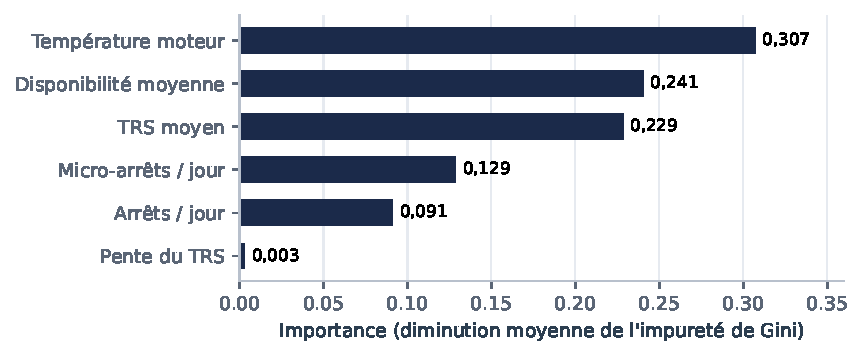
\includegraphics[width=0.78\textwidth]{figures/importances.pdf}
\caption{Importance des variables du modèle de risque.}
\label{fig:imp}
\end{figure}

La \textbf{température moteur} (0,307), la \textbf{disponibilité moyenne} (0,241) et le
\textbf{TRS moyen} (0,229) dominent, suivis des micro-arrêts et des arrêts. Ce classement est
cohérent avec l'analyse des corrélations et avec l'intuition métier : une machine qui chauffe et
s'arrête souvent est proche de la panne. La pente sur 5 jours n'apporte presque rien (0,003) :
calculée sur une fenêtre aussi courte, elle est dominée par le bruit journalier, alors que les
niveaux moyens sont plus stables.

Deux réserves s'appliquent : l'importance de Gini favorise les variables continues et se répartit
entre variables corrélées ; et, sur ce jeu simulé, la température est générée à partir de la perte
de disponibilité, ce qui explique en partie son rang.

\subsection{Score de risque actuel}
Pour chaque machine, le modèle est appliqué à la fenêtre la plus récente et la probabilité
$\hat p$ est traduite en niveau de risque : \textbf{faible} si $\hat p < 0{,}30$,
\textbf{modéré} si $0{,}30 \le \hat p < 0{,}60$, \textbf{élevé} si $\hat p \ge 0{,}60$.

\begin{table}[ht]
\centering\small
\caption{Risque de panne actuel par machine.}
\begin{tabular}{@{}lcc@{}}
\toprule
\textbf{Machine} & \textbf{Probabilité de panne} & \textbf{Niveau} \\
\midrule
M-03 & \textbf{0,905} & \textcolor{rouge}{\textbf{élevé}} \\
M-01, M-02, M-04, M-05 & 0,000 & \textcolor{vert}{faible} \\
\bottomrule
\end{tabular}
\end{table}

M-03 est la seule machine signalée, ce qui est cohérent avec la prévision de tendance de la
section précédente : les deux modèles convergent. Les probabilités nulles des autres machines
traduisent un modèle très tranché, conséquence du faible nombre de cas positifs ; sur données
réelles, une calibration des probabilités serait nécessaire.

% =====================================================================
\section{Mise en œuvre logicielle}

\subsection{Architecture}
Le code sépare la logique métier de l'interface, ce qui permet de la réutiliser telle quelle dans
le notebook et dans l'application.

\begin{table}[ht]
\centering\small
\caption{Organisation du code (Python 3.10+).}
\begin{tabularx}{\textwidth}{@{}l X@{}}
\toprule
\textbf{Fichier} & \textbf{Rôle} \\
\midrule
\code{calcul\_trs.py} & nettoyage, calcul de $D$, $P$, $Q$ et du TRS, synthèse par machine \\
\code{prediction.py} & prévision par régression, construction des variables, entraînement,
                       évaluation et score de risque \\
\code{maintenance\_predictive\_TRS.ipynb} & exploration, entraînement, évaluation ;
                       export du modèle dans \code{modele\_risque.joblib} \\
\code{app.py} & tableau de bord Plotly Dash (5 pages) \\
\code{generer\_donnees.py} & génération du jeu simulé \\
\bottomrule
\end{tabularx}
\end{table}

Le modèle exporté par le notebook est un dictionnaire \code{joblib} contenant le modèle entraîné,
la liste des variables, la taille de fenêtre, l'horizon et le seuil de panne. Le tableau de bord le
charge au démarrage ; s'il est absent, le modèle est entraîné à la volée avec les mêmes paramètres.

\subsection{Tableau de bord}
L'application Dash comporte cinq pages : vue d'ensemble, ingestion (import d'un CSV avec
validation du schéma), préparation (rapport de qualité), analyse du TRS (graphiques liés :
sélectionner une machine la met en avant dans tous les graphiques) et prédiction (risque par
machine, prévision, métriques). La vue d'ensemble déclenche une alerte lorsqu'une machine présente
un risque modéré ou élevé (figure~\ref{fig:app}).

\begin{figure}[ht]
\centering
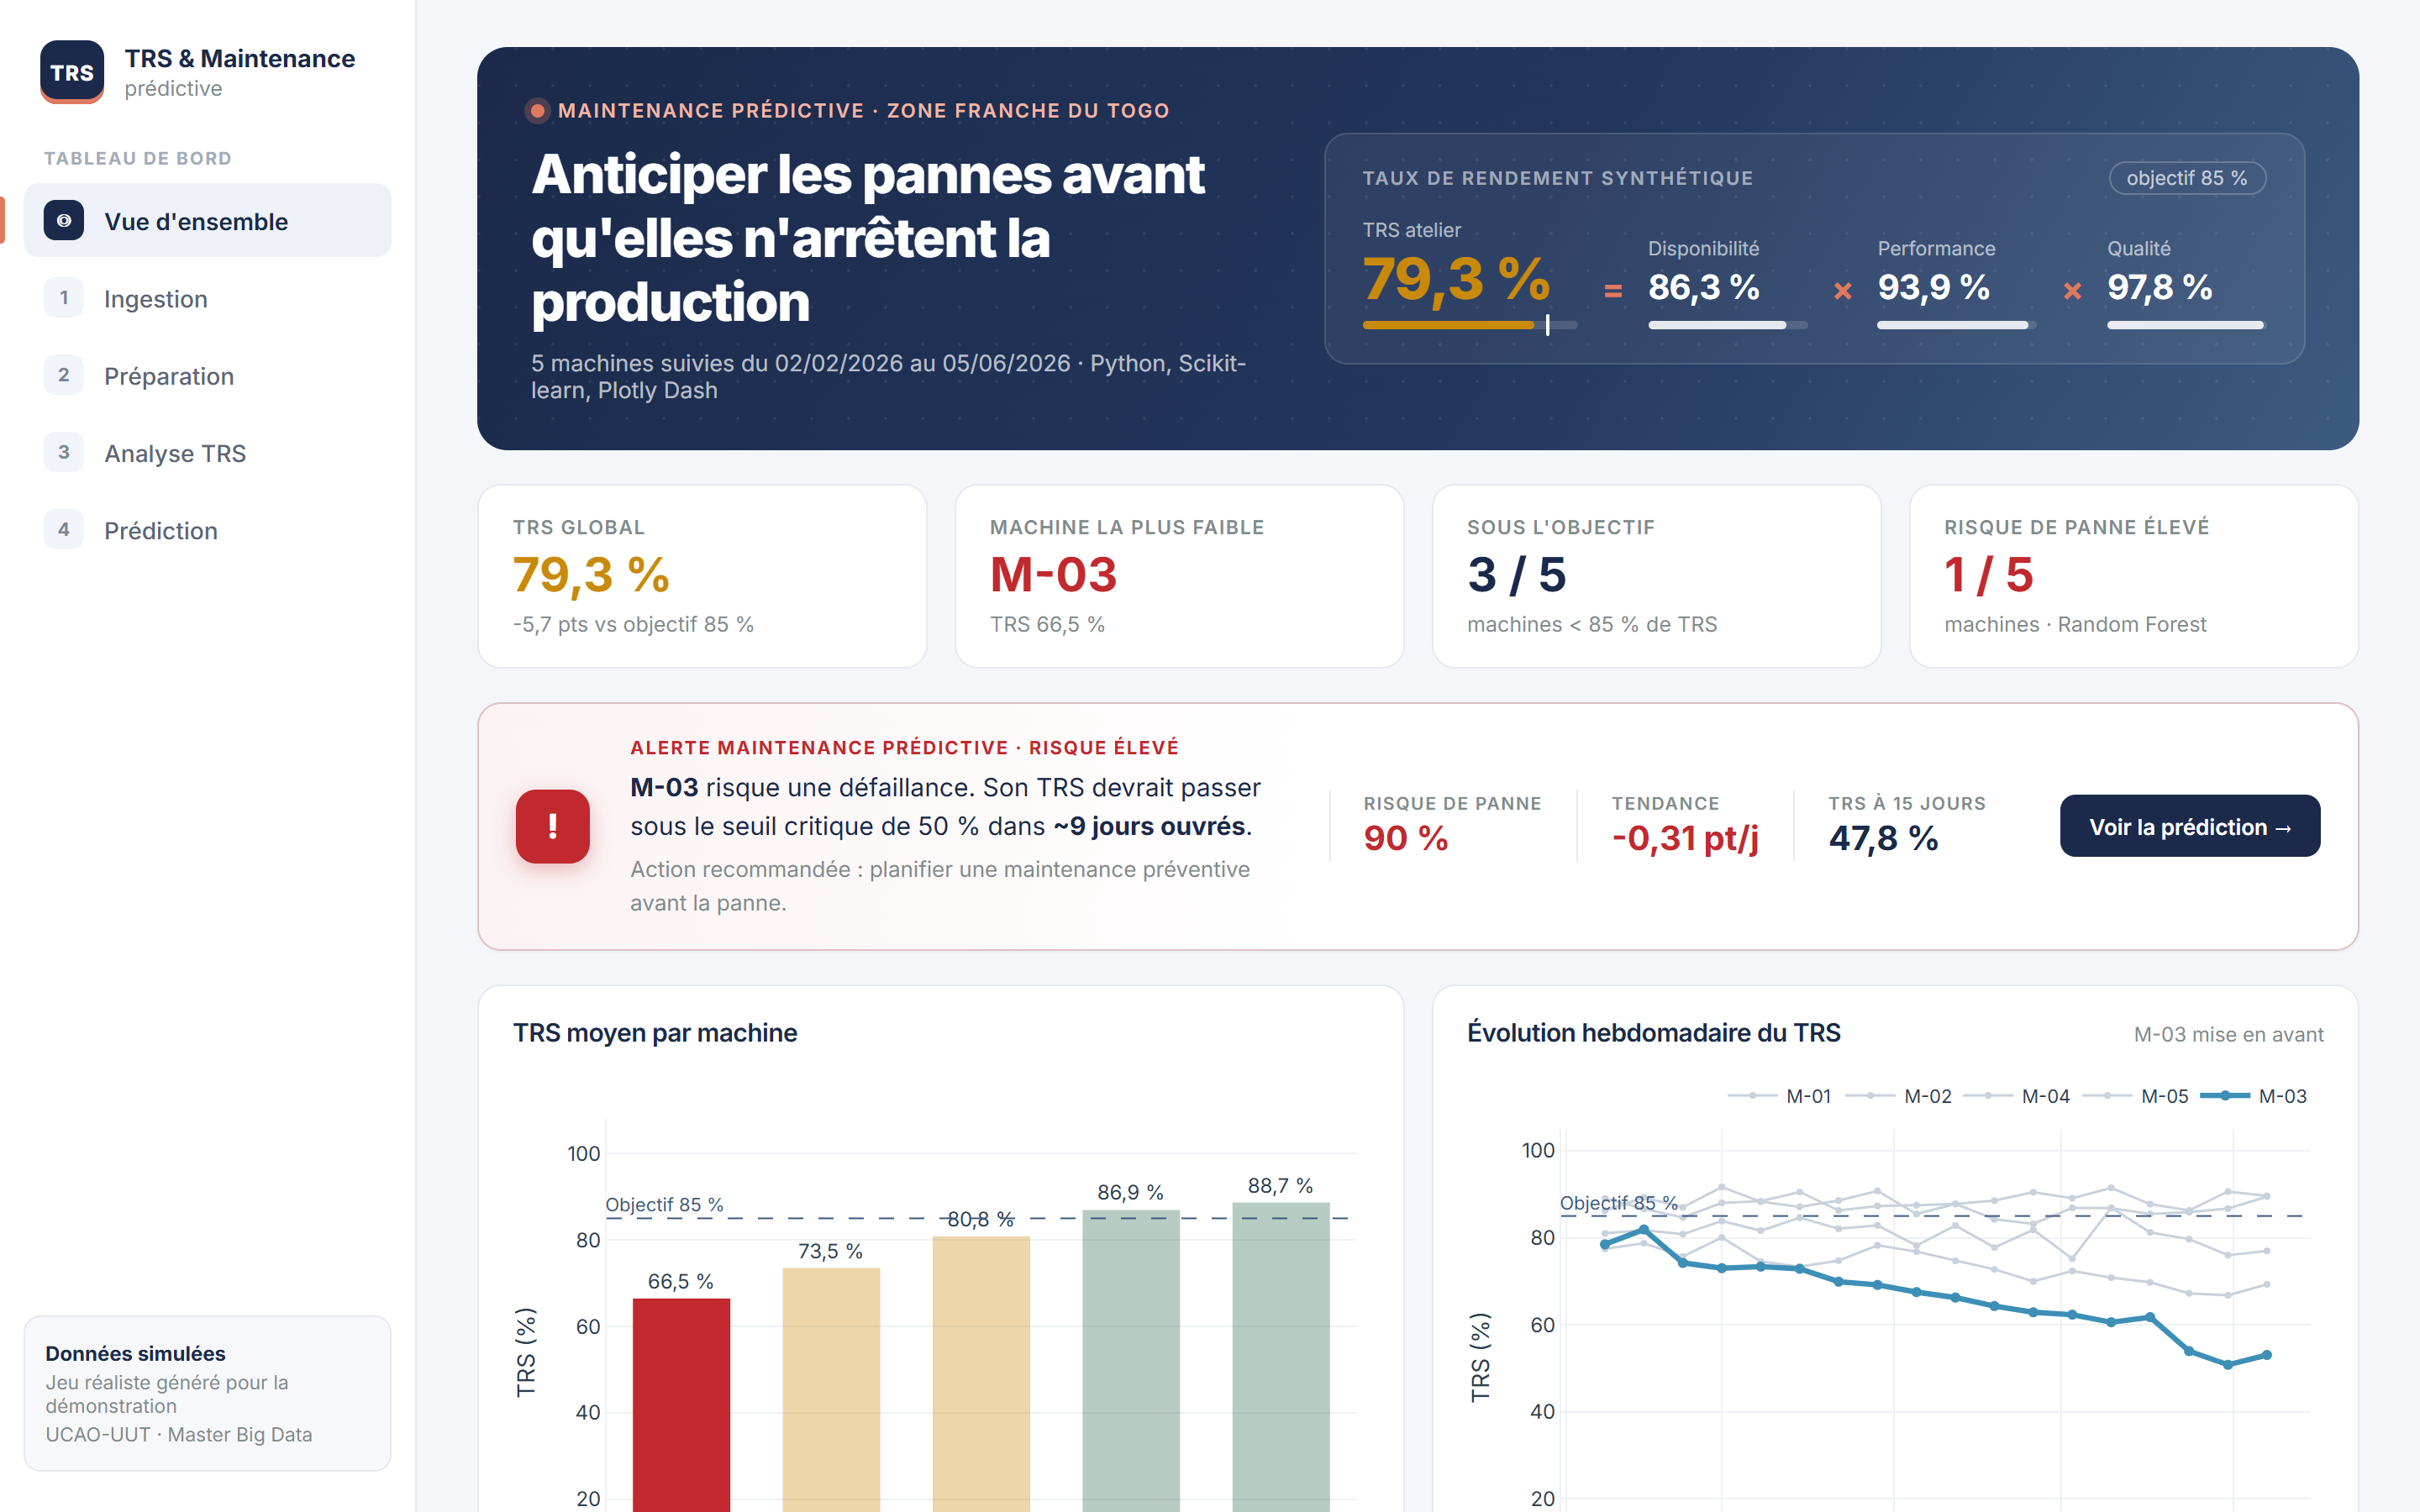
\includegraphics[width=\textwidth]{figures/vue_ecran.png}
\caption{Vue d'ensemble du tableau de bord : TRS décomposé, indicateurs et alerte de maintenance
prédictive sur M-03.}
\label{fig:app}
\end{figure}

\begin{figure}[ht]
\centering
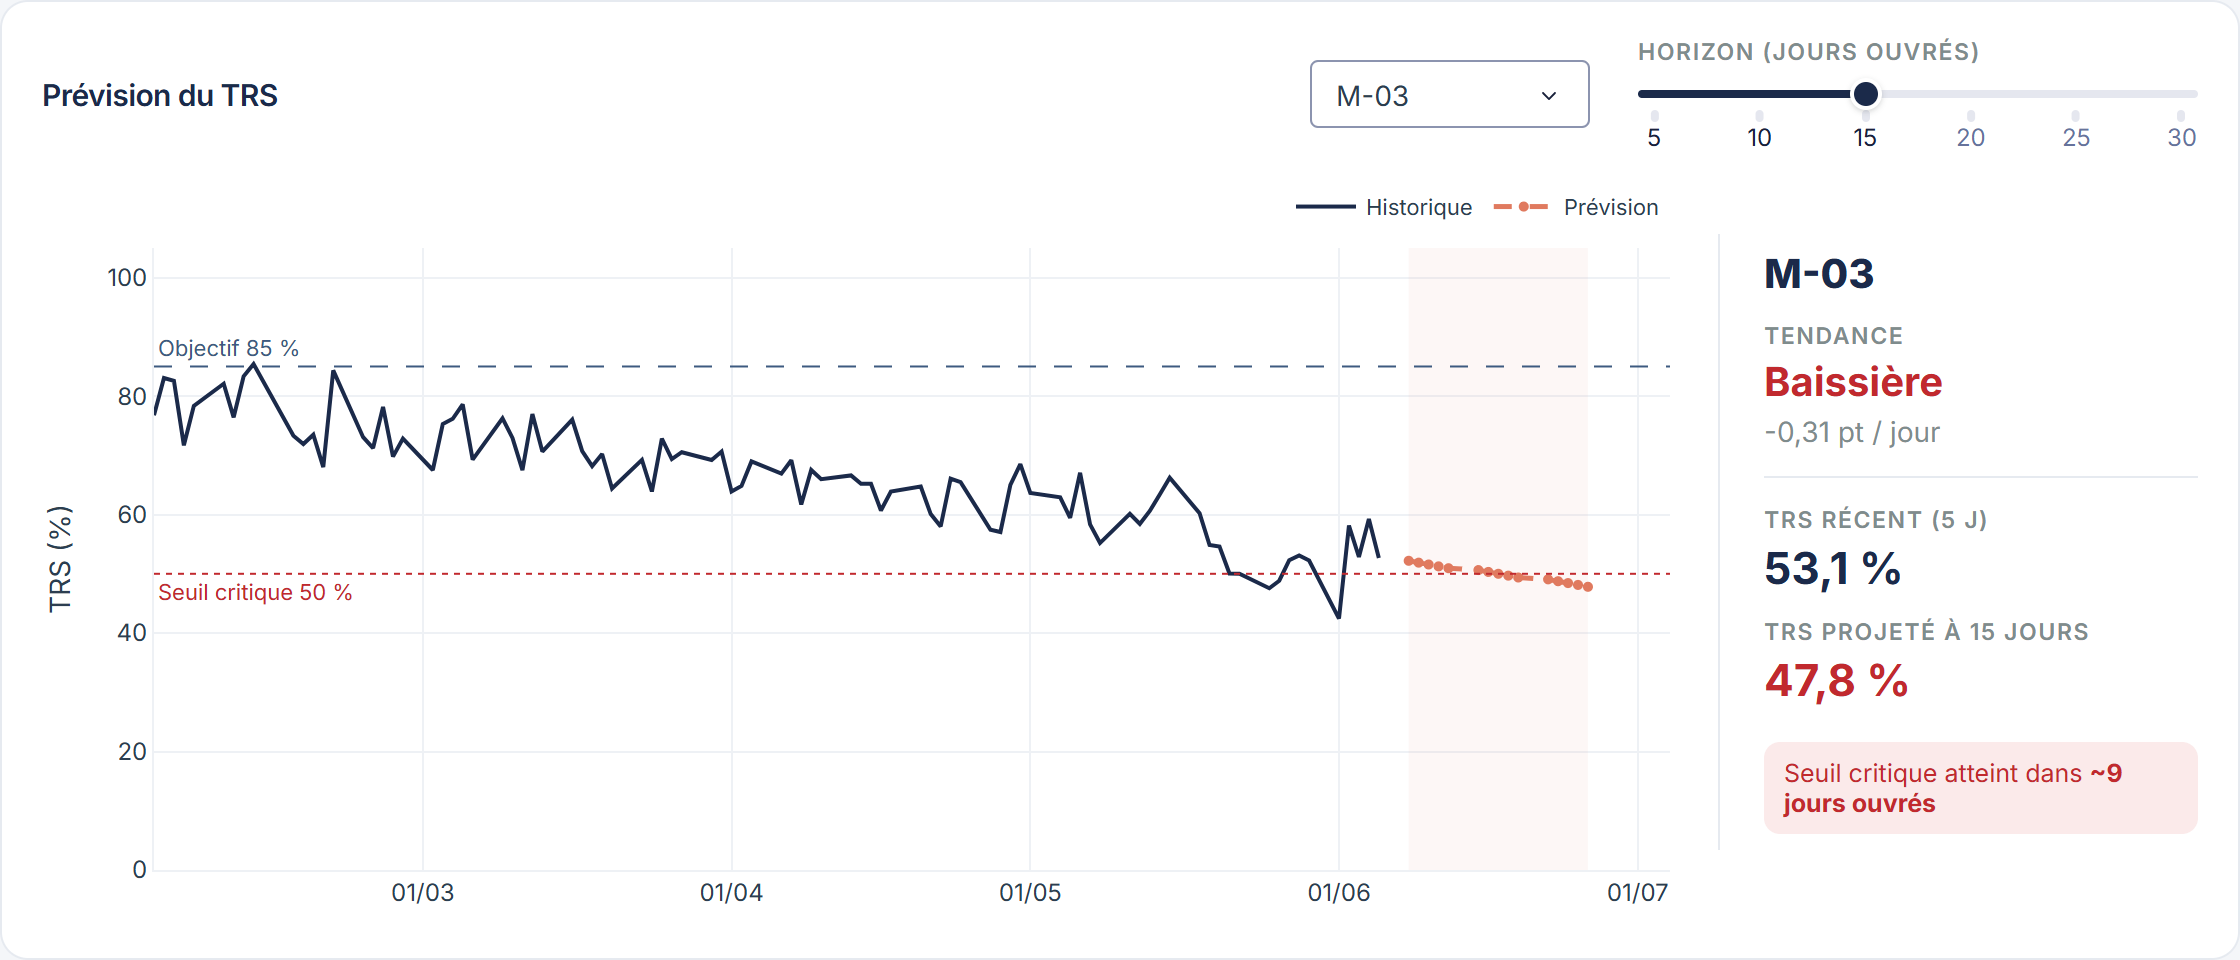
\includegraphics[width=0.92\textwidth]{figures/pred_prevision.png}
\caption{Page Prédiction : prévision du TRS de M-03 et délai estimé avant le seuil critique.}
\end{figure}

% =====================================================================
\section{Limites et perspectives}
\label{sec:limites}

\paragraph{Données simulées.} Les relations entre signaux d'usure et disponibilité sont définies
par le générateur ; le modèle les retrouve donc plus facilement que sur des données réelles,
bruitées et incomplètes. La principale perspective est l'application à des données d'usine, que
l'outil accepte déjà (import CSV avec validation du schéma).

\paragraph{Très peu d'événements.} Les 9 cas positifs proviennent de 3 journées de panne d'une
seule machine, et les fenêtres glissantes qui se chevauchent sont fortement corrélées entre elles.
Les métriques reposent donc sur très peu d'événements indépendants et doivent être lues comme
indicatives.

\paragraph{Découpage aléatoire de séries temporelles.} Des fenêtres voisines dans le temps peuvent
se retrouver l'une dans l'apprentissage, l'autre dans le test : l'évaluation est alors optimiste.
Un découpage chronologique (apprendre sur le passé, tester sur le futur) serait plus rigoureux,
mais il est impossible ici : toutes les pannes surviennent après le 28/04/2026, si bien qu'un
découpage \pct{70}/\pct{30} dans le temps laisse l'apprentissage sans aucune panne. Sur données
réelles, on utilisera une validation temporelle (\code{TimeSeriesSplit}) et une validation par
machine (\code{GroupKFold}) pour vérifier que le modèle se généralise à une machine non vue.

\paragraph{Pistes d'amélioration.}
\begin{itemize}
  \item choisir le seuil de décision en fonction des coûts réels (coût d'une panne contre coût
        d'une intervention), sur un jeu de validation ;
  \item rééquilibrer les classes (sur-échantillonnage SMOTE, sous-échantillonnage) et calibrer les
        probabilités ;
  \item enrichir les signaux (vibrations, consommation électrique, historique d'interventions) ;
  \item remplacer la tendance linéaire par des modèles de séries temporelles (ARIMA, lissage
        exponentiel) fournissant des intervalles de confiance ;
  \item comparer la forêt aléatoire à d'autres modèles (régression logistique, gradient boosting).
\end{itemize}

% =====================================================================
\section{Conclusion}
Ce projet met en place une chaîne complète, de la donnée brute de production à la prédiction, et la
restitue dans un tableau de bord utilisable par un responsable de production. Sur le scénario
simulé, les deux modèles convergent vers la même conclusion : la machine M-03, pénalisée par sa
disponibilité, se dégrade d'environ 0,3 point de TRS par jour et présente un risque de panne élevé,
ce qui laisse environ deux semaines pour planifier une intervention.

L'évaluation montre aussi les limites d'un apprentissage sur des événements rares : l'exactitude
est trompeuse, le seuil de décision doit être adapté au coût d'une panne manquée, et la fiabilité
des métriques dépend du nombre de pannes observées. Ces constats fixent la suite du travail :
confronter l'outil à des données réelles et en valider les performances dans le temps.

% =====================================================================
\appendix
\section{Reproduire les résultats}
\begin{tcolorbox}[colback=fond,colframe=fond,arc=2pt,left=8pt,fontupper=\ttfamily\footnotesize]
git clone https://github.com/kkepiphane/trs-zone-franche-tg.git\\
cd trs-zone-franche-tg\\
pip install -r requirements.txt\\[4pt]
python generer\_donnees.py \hfill\textrm{\color{muted}\# données simulées}\\
jupyter notebook maintenance\_predictive\_TRS.ipynb \hfill\textrm{\color{muted}\# entraînement, export}\\
python app.py \hfill\textrm{\color{muted}\# tableau de bord : http://127.0.0.1:8050}\\
python docs/rapport/generer\_figures.py \hfill\textrm{\color{muted}\# figures de ce rapport}
\end{tcolorbox}

Toutes les sources d'aléa sont fixées : la graine \code{42} est utilisée pour la génération des
données, pour la séparation apprentissage / test et pour la forêt aléatoire. Les chiffres de ce
rapport sont donc reproductibles à l'identique.

\end{document}
